\documentclass[12pt,a4paper]{article}
\usepackage[utf8]{inputenc}

\usepackage{mathtools}
\usepackage{amsmath}
\usepackage{amssymb}
\usepackage{amsthm}
\usepackage{amssymb}
\usepackage{mathdots}
\usepackage[pdftex]{graphicx}
\usepackage{fancyhdr}
\usepackage[margin=1in]{geometry}
\usepackage{multicol}
\usepackage{bm}
\usepackage{listings}
\usepackage{xcolor}
\usepackage{pdfpages}
\usepackage{algpseudocode}
\usepackage{tikz}
\usepackage{ulem}
\usepackage{enumitem}
\usepackage[T1]{fontenc}
\usepackage{inconsolata}
\usepackage{framed}
\usepackage{wasysym}
\usepackage[thinlines]{easytable}
\usepackage{hyperref}
\usepackage{minted}
\usemintedstyle{perldoc}
\hypersetup{
    colorlinks=true,
    linkcolor=blue,
    filecolor=magenta,      
    urlcolor=blue,
}
\definecolor{codegreen}{rgb}{0,0.6,0}
\definecolor{codegray}{rgb}{0.5,0.5,0.5}
\definecolor{codepurple}{rgb}{0.58,0,0.82}
\definecolor{backcolour}{rgb}{0.95,0.95,0.92}
\lstdefinestyle{mystyle}{
    backgroundcolor=\color{backcolour},   
    commentstyle=\color{codegreen},
    keywordstyle=\color{magenta},
    numberstyle=\tiny\color{codegray},
    stringstyle=\color{codepurple},
    basicstyle=\ttfamily,
    breakatwhitespace=false,         
    breaklines=true,                 
    captionpos=b,                    
    keepspaces=true,                 
    numbers=left,                    
    numbersep=5pt,                  
    showspaces=false,                
    showstringspaces=false,
    showtabs=false,                  
    tabsize=4
}
\lstset{style=mystyle}
\newcommand\numberthis{\addtocounter{equation}{1}\tag{\theequation}}
\newcommand{\rightqed}{
\begin{flushright}
$\blacksquare$
\end{flushright}
}
\newcommand\redsout{\bgroup\markoverwith{\textcolor{red}{\rule[0.5ex]{2pt}{0.4pt}}}\ULon}
\newcommand{\solution}{\noindent\textbf{Solution:}\\\indent}
\usepackage{graphics}
\usepackage{subfig}
\graphicspath{ {./images/} }

\title{6470 Algorithms Homework 4}
\author{Kushajveer Singh}
\date{}

\begin{document}
\maketitle

\subsection*{Problem 1}
\solution
(1) Proof by contradiction

Suppose $A$ is the optimal solution for the given Fractional Knapsack problem. Let $i$ and $j$ be two items with densities $d_i > d_j$. Suppose A contains $x$ units of $i\ (x < w_i)$ and $y$ units of $j\ (y \leq w_j\ and\ y = w_i - x)$.

We are left with $w_i - x$ grams of item $i$. And we know that the value per gram of this is $\frac{u_i}{w_i}$ and the value per gram of item $j$ with weight $y$ is $\frac{u_j}{w_j}$. The value of $y$ units of item $j$ is thus $\frac{u_j}{w_j}y$ and the value of $w_i-x$ grams of item $i$ is $\frac{u_i}{w_i}(w_i-x)$. 


We know $d_i > d_j$, which implies $\frac{u_i}{w_i}(w_i-x) > \frac{u_j}{w_j}$. This is a contradiction, because $A$ is the optimal solution and it must include the $x$ grams of item $i$ before using item $j$.

(2) Proof by "swapping technique"

Suppose A is the optimal solution for the given Fractional Knapsack problem. Let $i$ and $j$ be two items with densities $d_i > d_j$. We need to check if one gram of item $i$ belongs to A (and then we can repeat the reasoning till all grams of item $i$ are used).

Case 1: 1 gram of item $i \in A$. The above claim is proved.

Case 2: 1 gram of item $j \not\in A$. Suppose we use 1 gram of item $j$ to fill the space. The value of 1 gram of item $i$ is $\frac{u_i}{w_i}$ and value of 1 gram of item $j$ is $\frac{u_j}{w_j}$ and we are given $\frac{u_i}{w_i} > \frac{u_j}{w_j}$. This means A is not the optimal solution. To make the solution optimal we need to remove 1 gram of item $j$ with 1 gram of item $i$.

\subsection*{Problem 2}
\solution
(1) Suppose we are given $N$ light poles and each light pole can cover a radius of $r_i$ feet. Each light pole will light $2r_i$ feet. We want to determine the minimum number of light poles required to light $m$ feet.

The following is the DP solution for the given problem
\begin{equation*}
    L(k,M) = \min\begin{cases}
        L(k-1, M-2r_k) + 1 & m \geq 2r_k \\
        L(k-1, M) & 
    \end{cases}
\end{equation*}

with base case $L(0,M) = 0$ and $L(k,0) = 0$.

This problem has a greedy-choice property i.e. always choose the lamp that has the largest radius.

So there is an optimal solution that contains a light pole at position ($r_0, 2r_0 + r_1, 2r_0 + 2r_1 + r_2, \hdots$), where $r_0 \geq r_1 \geq r_2 \geq \hdots$.

(2) Suppose A is the optimal solution for the given problem and we are given two lamps with radius $r_i$ and $r_j$ with $r_i > r_j$. There are two options

Case 1: $r_i \in A$, the claim in (1) is proved.

Case 2: $r_i \not\in A$. Let $r_j \in A$, the lamp with the largest radius after $r_i$. Let all the lamps in $A$ cover a total of $x$ feet. If we used lamp $r_i$ instead of $r_j$, then $x-2r_j+2r_i$ feet would be covered. It is easy to check that $x-2r_j+2r_i > x$ as $r_i > r_j$, which means $A$ is not the optimal solution. So we need to swap $r_j$ with $r_i$ to make the solution optimal.

\newpage
\subsection*{Problem 3}
\solution

(1) The execution of Prim's algorithm is shown in the table below. Every cell represents the (key, parent) of the node. And the node that is dequeued in the current step is shown with a red line and the nodes not in the priority queue are shown with a black line. \\

\begin{tabular}{|c|c|c|c|c|c|c|c|}
\hline
\textbf{Step} & \textbf{a} & \textbf{b} & \textbf{c} & \textbf{d} & \textbf{e} & \textbf{f} & \textbf{z} \\
\hline
\textbf{Initialize} & ($\infty$, N) & ($\infty$, N) & ($\infty$, N) & ($\infty$, N) & ($\infty$, N) & ($\infty$, N) & ($\infty$, N) \\
\hline
\textbf{Root init} & ($\infty$, N) & ($\infty$, N) & (0, N) & ($\infty$, N) & ($\infty$, N) & ($\infty$, N) & ($\infty$, N) \\
\hline
\textbf{Deque c} & (3, c) & ($\infty$, N) & \redsout{(0, N)} & (7, c) & (10, c) & ($\infty$, N) & ($\infty$, N) \\
\hline
\textbf{Deque a} & \redsout{(3, c)} & (4, a) & \sout{(0, N)} & (7, c) & (10, c) & ($\infty$, N) & ($\infty$, N) \\
\hline
\textbf{Deque b} & \sout{(3, c)} & \redsout{(4, a)} & \sout{(0, N)} & (7, c) & (10, c) & (5, b) & ($\infty$, N) \\
\hline
\textbf{Deque f} & \sout{(3, c)} & \sout{(4, a)} & \sout{(0, N)} & (7, c) & (10, c) & \redsout{(5, b)} & (16, N) \\
\hline
\textbf{Deque d} & \sout{(3, c)} & \sout{(4, a)} & \sout{(0, N)} & \redsout{(7, c)} & (2, d) & \sout{(5, b)} & (16, N) \\
\hline
\textbf{Deque e} & \sout{(3, c)} & \sout{(4, a)} & \sout{(0, N)} & \sout{(7, c)} & \redsout{(2, d)} & \sout{(5, b)} & (5, e) \\
\hline
\textbf{Deque z} & \sout{(3, c)} & \sout{(4, a)} & \sout{(0, N)} & \sout{(7, c)} & \sout{(2, d)} & \sout{(5, b)} & \redsout{(5, e)} \\
\hline
\end{tabular} \\

From the above table
\begin{itemize}
    \item Red line: indicates when a vertex is dequeued from Q
    \item Black link: Indicates vertices that are not in Q
    \item ($\infty, N)$: Means vertex has key = infinity and parent = NULL
    \item A new edge is included into the partially constructed spanning tree, when the node dequeued from Q has a parent pointer not equal to NULL. This means when we deque $a$, the edge $(c,a)$ is added to the spanning tree. And the same goes for when we deque $b,f,d,e,z$.
\end{itemize}

MST for the given graph includes the following edges
\begin{equation*}
    (a,c), (a,b), (b,f), (c,d), (d,e), (e,z)
\end{equation*}

(2) Suppose we dequeued vertex $a$ from Q and updated the weight of its neighbors. Now suppose after some steps we deque vertex $b$ from Q (where $b$ is the neighbor of $a$). To show Prim's algorithm does not need to check if a cycle is formed when adding a new edge it is sufficient to show that for the above situation Prim's algorithm would never consider the edge $(a,b)$ (because when we deque a vertex from Q, we add the corresponding edge (vertex, vertex.parent) to the partially constructed spanning tree and a cycle can only be formed if two neighboring vertices are connected).

From line 9 of the algorithm discussed in class i.e. ($if\ v\in Q\text{ and } w(u,v) < v.key$), we note that the neighbor of vertex $b$ (i.e. $a$) would never be considered as we have already dequeued it from the priority queue, which means the edge $(a,b)$ would never be considered. Due to this reason, Prim's algorithm does not need to check if it would form a cycle when a new edge is included.

\subsection*{Problem 4}
\solution
(1) \\

\begin{tabular}{c|c}
    \textbf{Edge} & \textbf{Sets} \\
    \hline
    & [a] [b] [c] [d] [e] [f] [z] \\ \\
    (d,e) & [a] [b] [c] \underline{[d]} \underline{[e]} [f] [z] \\
    & [a] [b] [c] [d, e] [f] [z] \\ \\
    (a,c) & \underline{[a]} [b] \underline{[c]} [d, e] [f] [z] \\
    & [a, c] [b] [d, e] [f] [z] \\ \\
    (a,b) & \underline{[a, c]} \underline{[b]} [d, e] [f] [z] \\
    & [a, b, c] [d, e] [f] [z] \\ \\
    (b,f) & \underline{[a, b, c]} [d, e] \underline{[f]} [z] \\
    & [a, b, c, f] [d, e] [z] \\ \\
    (e,z) & [a, b, c, f] \underline{[d, e]} \underline{[z]} \\
    & [a, b, c, f] [d, e, z] \\ \\
    (c,d) & \underline{[a, b, c, f]} \underline{[d, e, z]} \\
    & [a, b, c, d, e, f, z] \\ \\
    (c,e) & \underline{[a, b, c, d, e, f, z]}\\
    & [a, b, c, d, e, f, z] \\ \\
    (b,e) & \underline{[a, b, c, d, e, f, z]}\\
    & [a, b, c, d, e, f, z] \\ \\
    (f,z) & \underline{[a, b, c, d, e, f, z]}\\
    & [a, b, c, d, e, f, z] \\ \\
\end{tabular}

In the above table, first column refers to the edge that is picked at each step and the second column stores the information of the sets.

For every edge, the corresponding sets are shown with an underline and if the the sets are disjoint, the sets are merged, otherwise the sets remain unchanged. In case the sets can be merged the edge is added to the partially constructed spanning tree.

The MST produced by Kruskals' algorithm contains the following edges
\begin{equation*}
    (d,e), (a,c), (a,b), (b,f), (e,z), (c,d)
\end{equation*}

(2) No we cannot simplify the implementation. If we run the proposed algorithm on the graph in Q3, we get a counterexample as shown below \\

\begin{tabular}{c|c}
    \textbf{Edge} & \textbf{Visited Nodes} \\
    \hline
    (d,e) & {d,e} \\
    (a,c) & {a,c,d,e} \\
    (a,b) & {a,b,c,d,e} \\
    (b,f) & {a,b,c,d,e,f} \\
    (e,z) & {a,b,c,d,e,f,z} \\
\end{tabular}

After running the algorithm for above edges, we cannot add new edges to the graph as all nodes have been visited once. And the graph produced by above edges is disconnected, so we cannot simplify the implementation by checking if both vertices $u$ and $v$ have already been in the partially constructed MST when the new edge $(u,v)$ is being considered.

\subsection*{Problem 4}
\solution
(1) The nodes are visited in the following order $C \rightarrow D \rightarrow E \rightarrow F \rightarrow A \rightarrow B$. The start and finish times are shown below

\begin{align*}
    A &= (9,10) \\
    B &= (11, 12) \\
    C &= (1,8) \\
    D &= (2,7) \\
    E &= (3,4) \\
    F &= (5,6)
\end{align*}

(2)

Tree Edges = $\{(c,d), (d,e), (d,f) \}$

Back Edges = $\{ \}$

Forward Edges = $\{(c,f), (c,e) \}$

Cross Edges = $\{(a,c), (a,d), (b,c), (b,a), (f,e) \}$

(3) The nodes are visited in the following order $C \rightarrow A \rightarrow B \rightarrow D \rightarrow E \rightarrow F$.

Tree Edges = $\{(c,a), (a,b), (a,d), (d,e), (e,f) \}$

Back Edges = $\{(b,c), (d,c), (e,c), (f,c), (f,d) \}$

\newpage
\subsection*{Problem 6}
\solution
(1)

\begin{lstlisting}[mathescape=true]
DFS-Reachability(G,s,t)
    for $u \in V$ do
        u.visit = 0
    S = Stack()
    
    s.visit = 1
    push(s,S)
    while Not empty(S)
        u = top(S)
        if u = t; return "Yes"
        if $\exists v \in Adj[u]$ and v.visit = 0
            v.visit = 1
            push(v,S)
        else
            pop(S)
    
    return "No"
\end{lstlisting}

(2) Vertices that are in set R have $u.visit = 1$ set at initialization. This ensures these vertices are never visited.


\begin{lstlisting}[mathescape=true]
DFS-Reachability(G,R,s,t)
    for $u \in V$ do
        u.visit = 0
        if $u \in R$
            u.r = 1
            u.visit = 1
        else
            u.r = 0
    S = Stack()
    if s.r = 1 or t.r = 1
        return "No"
        
    s.visit = 1
    push(s,S)
    while Not empty(S)
        u = top(S)
        if u = t; return "Yes"
        if $\exists v \in Adj[u]$ and v.visit = 0
            v.visit = 1
            push(v,S)
        else
            pop(S)
    
    return "No"
\end{lstlisting}

\newpage
\subsection*{Problem 7}
\solution

Dijkstra's algorithm would fail to find the shortest path between $s$ and $t$ in the graph shown below.

\begin{figure}[H]
    \centering
    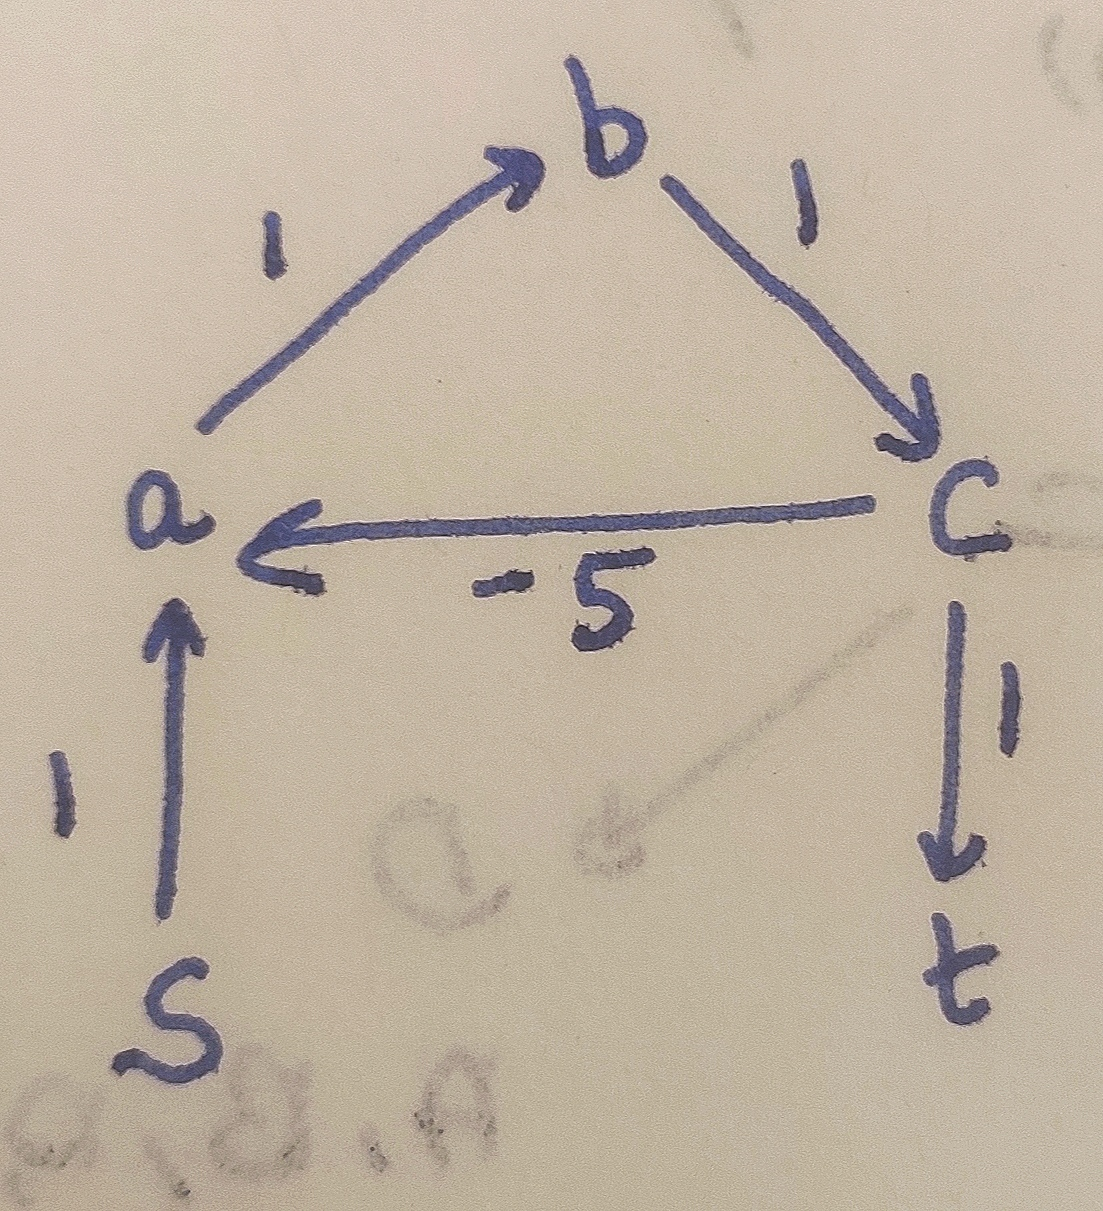
\includegraphics[width=7cm]{prob_7.jpg}
\end{figure}

During the execution of the algorithm, we use a priority where the minimum value is dequeued from the priority queue and due to this reason we only visit all the vertices only once. Due to this reason, Dijkstra's algorithm is not able to find negative cycles in the graph.

The shortest distance for the graph shown above contains infinite loops of $a \rightarrow c \rightarrow a$. Dijkstra's algorithm would return 4 as the shortest path distance in this case.

\subsection*{Problem 8}
\solution
\begin{align*}
    D^0 &= \begin{bmatrix}
        0 & \infty & \infty \\
        2 & 0 & -3 \\
        4 & 4 & 0
    \end{bmatrix} & P^0 &= \begin{bmatrix}
        0 & 0 & 0 \\
        0 & 0 & 0 \\
        0 & 0 & 0
    \end{bmatrix} \\
    D^1 &= \begin{bmatrix}
        0 & \infty & \infty \\
        2 & 0 & -3 \\
        4 & 4 & 0
    \end{bmatrix} & P^1 &= \begin{bmatrix}
        0 & 0 & 0 \\
        0 & 0 & 0 \\
        0 & 0 & 0
    \end{bmatrix} \\
    D^2 &= \begin{bmatrix}
        0 & \infty & \infty \\
        2 & 0 & -3 \\
        4 & 4 & 0
    \end{bmatrix} & P^2 &= \begin{bmatrix}
        0 & 0 & 0 \\
        0 & 0 & 0 \\
        0 & 0 & 0
    \end{bmatrix} \\
    D^3 &= \begin{bmatrix}
        0 & \infty & \infty \\
        1 & 0 & -3 \\
        4 & 4 & 0
    \end{bmatrix} & P^3 &= \begin{bmatrix}
        0 & 0 & 0 \\
        3 & 0 & 0 \\
        0 & 0 & 0
    \end{bmatrix}
\end{align*}


\end{document}
